%
% Draft  document dpcell.tex
% Analysis of data from ab46 on dermal papilla cell counts
%
 
\documentclass[titlepage]{article}  % Latex2e
\usepackage{graphicx,lscape,subfigure}
\usepackage{tikz}
\usepackage{bm,longtable}
\usepackage{textcomp}
 

\title{Dermal papilla cell counts and fibre diameter}
\author{Paul Swan Philip Moore and Neville Jackson}
\date{20 Oct 2021} 

 
\begin{document} 


 
\maketitle      
\tableofcontents

$\newcommand{\E}{\mathrm{E}}$
$\newcommand{\Var}{\mathrm{Var}}$
$\newcommand{\Cov}{\mathrm{Cov}}$ 
$\newcommand{\SD}{\mathrm{SD}}$ 

\clearpage
\section{Introduction} 
It has been shown that there  exists in the dermis of the the developing sheep foetus a population of cells, known as pre-papilla cells, which migrate to the site s of follicle formation and differentiate, ending up in the papilla of the follicle bulb ( Moore, etal (1989)~\cite{moor:89}, Moore etal (1998)~\cite{moor:98}). These cells are of mesenchymal origin, in contrast to all other tissue in the follicle, which arises from the epidermis. It is thought that these cells control follicle development, and, in particular, that the number of papilla cells which end up in a follicle bulb  at least partly determines follicle size and fibre diameter, and perhaps other follicle and fibre characteristics.

\section{Materials and Methods}

The sheep observed were from CSIRO single character selection lines described by Turner, Brooker and Dolling (1970)~\cite{turn:70}. Four lines were studied - high staple length, low staple length, high fibre diameter, amd low fibre diameter selection.  The sheep measured were born in 1971 to 1978 and were a random sample of the available animals. Measurements were on biopsy specimens and wool samples taken at 2 years of age.

Fibre diameter data were with the airflow technique (ref?)
Phil will have to do a methodology here !!

The observations made were
\begin{itemize}
\item dermal papilla cell count per follicle
\item dermal papilla cell count per $mm^{2}$
\item surface area of sheep (estimated from bodyweight) $m^{2}$
\item body weight (2 yrs) $Kg$
\item Np no of primaries per $mm^{2}$
\item Nps no of follicles per $mm^{2}$
\item Cww clean wool weight $Kg$
\item Cwwperua clean wool weight per unit area
\item Stal staple length $mm$
\item Staladj staple length adjusted to 365 days $mm$
\item Diam fibre diameter $\mu m$
\item Cww2 another clean wool weight $Kg$
\item Cww2adj clean wool weight adjusted to 365 days
\item SorT coding for single=1, twin=2
\item Hcap coding for handicap SPA=6, SPM=7, TPA=8, TPM=9
\item Line coded L+=1, L-=2, D+=5, D-=6 
\end{itemize}



\subsection{Statistical Methods}
Data were imported into the R statistical program~\cite{rprog:13} .

The regression relationship between dermal papilla cell count and diameter was estimated assuming nboth variables were subject to measurement error. Total least squares or orthogoinal regression was used. 

The effects of Line and SorT ( single or twin) in dermal papilla cell count per follicle was examined using analysis of variance and tables of means.

\section{Results}

 The average number of pre-papilla cells per follicle  is something for which we actually have some limited data. A sample of 42 sheep, from a CSIRO selection experiment with  4 lines selected for high and low fibre diameter and high and low staple length, were skin sampled and counts of dermal papilla cells per follicle bulb made. For 34 of these 42 sheep, an average fibre diameter measurement was available.

\subsection{ Dermal papilla cell number and fibre diameter}
 The relationship obtained between average number of dermal papilla cells per follicle and average fibre diameter is shown in Figure~\ref{fig:dpccdiam}
%\documentclass{article}
%\usepackage{graphicx,subfigure}
%\begin{document}

\begin{figure}[!h]
  \centering
   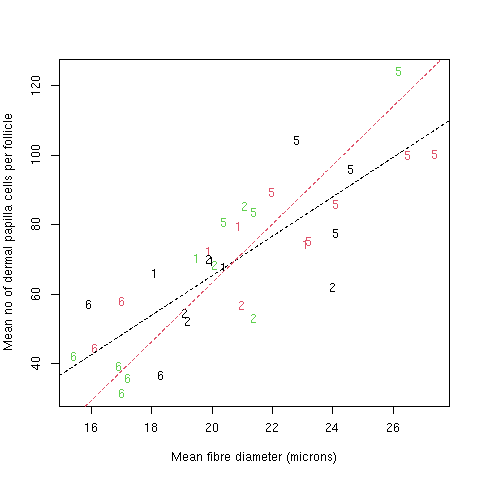
\includegraphics[width=0.9\textwidth]{dpccdiam2.png}
  \caption{Plot of mean fibre diameter against mean number of dermal papilla cells per follicle for 34 sheep from CSIRO selection experiments. The coloured numbers representing each point indicate the selection line (1 = high staple length, 2 = low staple length, 5 = high fibre diameter, 6 = low fibre diameter). The two dashed lines are   linear regressions of papilla cell count on diameter (black) and of diameter on papilla cell count (red).}
  \label{fig:dpccdiam}
\end{figure}

%\end{document}


In Figure~\ref{fig:dpccdiam} the black dashed regression line is obtained by regressing dermal papilla cell count on diameter. Its formula is
\begin{displaymath}
C = -48.2981 + 5.678 D
\end{displaymath}
where
\begin{description}
\item[C] is dermal papilla cell count per follicle
\item[D] is mean fibre diameter
\end{description}
The red dashed line is obtained by regressing diameter on dermal papilla cell count. Its formula is
\begin{displaymath}
D = 12.5031 + 0.1184 C
\end{displaymath}
which when reversed to put C on the Y-axis becomes
\begin{displaymath}
C = -105.6005 + 8.4459 D
\end{displaymath}
The issue with these regressions is that both dermal papilla cell count and diameter are variables with measurement and sampling errors. Classical regression assumes the variate on the X-axis is known without error. So neither of the above regressions is appropriate as a calibration to predict diameter from dermal papilla cell count. 

The correct approach is to use total least squares regression ( also known as orthogonal regression) . When we do orthogonal regression we get 
\begin{displaymath}
C = -104.3949 + 8.386858 D
\end{displaymath}
which is so close to the red dashed line that it plots on top of it. 
So this is our formula for diameter prediction, we just have to reverse transform it to get 
\begin{displaymath}
D = 12.44744 + 0.119234 C 
\end{displaymath}


Why is the orthogonal regression closer to one of the simple regressions?  Because one variable has more error than the other.  The orthogonal regression bisects the two simple regressions in proportion to the relative size of their error variances.


\subsection{Dermal papilla cell number and cross sectional area}
Relating dermal papilla cell number to diameter as in the previous section is a kludge. Theoretically dermal papilla cell number should relate to cross sectional area of fibres, so using diameter makes a scale mismatch. We estimate average fibre cross sectional area as
\begin{displaymath}
A = \frac{\pi}{4} D^{2}
\end{displaymath}
This ignores the contribution which variance of diameter makes to mean cross sectional area. We can not do anything to allow for variance because the data does not include variance of diameter.
The relationship between dermal papilla cell number and cross sectional area is shown in Figure~\ref{fig:dpca}
%\documentclass{article}
%\usepackage{graphicx,subfigure}
%\begin{document}

\begin{figure}[!h]
  \centering
   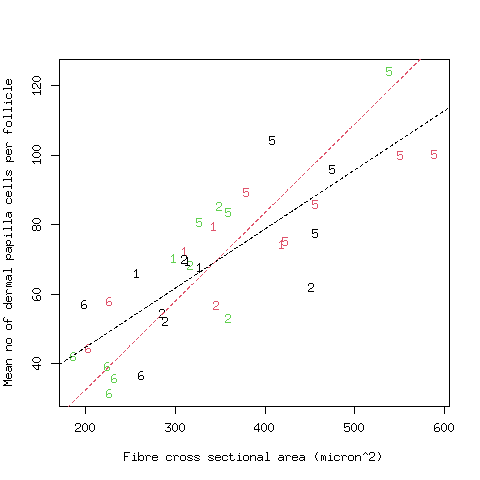
\includegraphics[width=0.9\textwidth]{dpcca.png}
  \caption{Plot of mean fibre cross sectional area against mean number of dermal papilla cells per follicle for 34 sheep from CSIRO selection experiments. The coloured numbers representing each point indicate the selection line (1 = high staple length, 2 = low staple length, 5 = high fibre diameter, 6 = low fibre diameter). The two dashed lines are   linear regressions of papilla cell count on cross sectional area (black) and of cross sectional area on papilla cell count (red).}
  \label{fig:dpca}
\end{figure}

%\end{document}


In Figure~\ref{fig:dpca} The black dashed regression line is obtained by regressing dermal papilla cell number on cross sectional area. Its formula is
\begin{displaymath}
C = 10.82950 + 0.16980 A
\end{displaymath}
where
\begin{description}
\item[C] is dermal papilla cell count per follicle
\item[A] is estimated mean fibre cross sectional area
\end{description}

The red dashed regression line is obtained by regressing cross sectional area on dermal papilla cell count. Its formula is
\begin{displaymath}
A = 72.2312 + 3.9270 C
\end{displaymath}
which when transposed to put C on the Y-axis becomes
\begin{displaymath}
C = -18.39348 + 0.2546473 A
\end{displaymath}

The correct approach is to use total least squares regression ( also known as orthogonal regression) . When we do orthogonal regression we get
\begin{displaymath}
C = 9.99927+ 0.172209 A
\end{displaymath}
which is so close to the black dashed line that it plots on top of it.
So this is our best formula for cross sectional area prediction, we just have to reverse transform it to get

\begin{displaymath}
A = -58.06468 + 5.80689 C
\end{displaymath}


Why is the orthogonal regression on cross sectional area similar to the blask dashed line but orthogonal regression on diameter close the red dashed line?  Because changing from diameter to cross sectional area has altered the balance of errors between the two variates by changing the scaling.  Cross sectional area has a larger mean and variance than diameter. 


\subsection{Line and SorT effects on dermal papilla cell number}
A model was fitted as follows
\begin{verbatim}
> aov2.dpcc <- aov(Dpccperfoll ~ SorT + Line + 1, data = dpcc.df)
> summary(aov2.dpcc)
            Df Sum Sq Mean Sq F value   Pr(>F)    
SorT         1    624     624    4.74   0.0381 *  
Line         3  11094    3698   28.10 1.36e-08 ***
Residuals   28   3684     132                     
---
Signif. codes:  0 ‘***’ 0.001 ‘**’ 0.01 ‘*’ 0.05 ‘.’ 0.1 ‘ ’ 1
9 observations deleted due to missingness
\end{verbatim}
 This shows that Line differences were highly significant and  SorT effects were marginally significant.
The effects (deviations from the overall mean) for Line and SorT were
\begin{verbatim}
> model.tables(aov2.dpcc)
Tables of effects

 SorT 
         1      2
     3.505 -5.392
rep 20.000 13.000

 Line 
       1      2     5      6
    1.78 -6.006 21.53 -25.91
rep 7.00  7.000 11.00   8.00
\end{verbatim}
  The big difference is between D+ and D- Lines (coded 5 and 6). If diameter is related to dermal papilla cell count as we assert, one would expect selection for diameter to alter dermal cell papilla count. It has.

 Twins (coded 2 for SorT) have a lower dermal papilla cell count. Twins also have a lower diameter. This is a bit more problematic. Twins have lower growth and therefore probably have a smaller population of pre-papilla cells for aggregates to form from (bad english). Why Twins would form aggregates with fewer cells is a mystery, unless one assumes aggregate formation is affected by the size of the population of unaggregated cells. That is something we need to think about.
 
\section{Discussion}
There is other published data on dermal papilla cell numbers in follicles of other species. In mice, Chi, Wu, and Morgan(2013)~\cite{chi:13} observe that dermal papilla cell numbers vary between 20 and 100 per follicle, with guard hairs having more than other fibre types, and Zigzag fibres least. This agrees with our adult sheep estimates. The papilla cell numbers fluctuated with the mouse hair cycle, and their variation correlated with hair length and diameter. So the number of dermal papilla cells is not fixed for the life of a follicle, it can fluctuate with the hair cylcle, and fibre dimensionss fluctuate with it. Sheep are different from mice in that most of their follicles are in Anagen for long periods.  What we need to note here is a caution that adult dermal papilla cell numbers per follicle are not necessarily the numbers of pre-papilla cells used to initially form the follicle.

Things other than dermal papilla cell count affect observed mean fibre diameter. We need to refer to Dry's concepts of {\em base} and {\em check} in birthcoats. {\em Base} is the diameter a follicle would grow if there were no other follicles around it sharing resources. {\em Check} is the diameter actually observed from follicles suffering some degree of {\em check} due to the surrounding follicles in the trio group. 

Dermal cell papilla count controls base diameter (ie maximum potential diameter). It does this by controlling the overall potential size of the follicle, the follicle bulb, and the fibre, not by controlling the partitioning of differentiating bulb cells between the inner root sheath and the fibre. See Jackson, Swan, and Watts (2018)~\cite{jack:18}  full presentation of the maths of how a follicle controls fibre length growth rate and fibre diameter.

Our regression equation estimates {\em checked diameter} because the diameter data used to fit the regressions are checked diameters. We do not know how much {\em check} there is in these data. We may just  assume it is some percentage of the unknown {\em base diameter}.

The only place where {\em base diameter} can be directly observed is in the birthcoat. The coarse curved sickle tips on Pc fibres are the unchecked diameter of fibres growing in utero from Pc follicles, with no other follicles around them to provide a {\em check} and probably an ample nutrient supply. They are indeed coarse, except in SRS Merinos (and in Wensleydales), and from this we suggest that SRS Merinos have small numbers of papilla cells in primary follicles.  

As far as predicting diameter goes, our equation gives an estimate of {\em checked diameter} at the average degree of check existing in the sheep used to fit the equation. We may be able to apply some estimate of 'percentage of check' which would presumably come from considerations of intra-trio-group-density and nutrition.

There is a well known across breed relationship between diameter and density. See Figure 11 on page 26 of Jackson (2017)~\cite{jack:17b} which shows data from Carter(1968)~\cite{cart:68} with breed means for Dp plotted against breed means for S/P ratio. The dramatic fall in Dp as S/P ratio increases is evidence of the {\em check} effect, Dp is reduced in the presence of increasing numbers of secondary follicles in the trio group.  Modern Merino sheep are fine because of the {\em check} effect of increasing numbers of secondary follicles, with the possible exception of SRS Merinos, which also have a lower {\em base} ie a lower number of dermal papilla cells per follicle.

There is also variation between follicles within an individual sheep. That is all dpcc, ie all {\em base}.  The density and the nutrition are same for all follicles within a sheep except for minor body variations. So diameter distribution within a fleece is all {\em base}. That gives us some hope that we can understand diameter distribution within a fleece purely by studying random variation in the numbers of dermal papilla cells in follicles. Another document (dpcpoisson.pdf) looks at using sampling from a Poisson distribution to emulate the distribution of dermal papilla cell numbers across follicles.

Everything we have said in Discussion about diameter applies equally to cross sectional area. Our regression equation predicts checked cross sectional area, at the average level of check applying in our data set. We do not at this stage know how to predict maximum or potential diameter or cross sectional area, even though we know that {\em base or maximim or potential} is what number of papilla cells actually determines.



\clearpage
\begin{thebibliography}{99}

\bibitem{bogo:40}
 Bogolyubsky S.N. (1940) cited by Fraser A.S and Short B.F. (1960) The Biology of the Fleece. Animal Research Laboratories Technical Paper No 3. CSIRO Melbourne 1960.


\bibitem{cart:43}
Carter H.B. (1943) Studies in the biology of the skin and fleece of sheep. 1. The development and general histology of the follicle group in the skin of the Merino. 2. The use of tanned sheepskin in the study of follicle population density. 3. Notes on the arrangement, nomenclature, and variation of skin folds and wrinkles in the Merino. C.S.I.R. Bulletin No 164, Melbourne, 1943

\bibitem{cart:55}
Carter, H.B. (1955) The hair follicle group in sheep Animal Breeding Abstracts 23(2) 101-116

\bibitem{cart:68}
Carter,H.B. (1968) Comparative Fleece Analysis Data for Domestic Sheep. The Principal Fleece Staple Values of Some Recognised Breeds. Agricultural Research Council, 1968

\bibitem{chi:13}
Chi, W., Wu, E., and MOrgan, B.A. (2013) Dermal papilla cell number specifies hair size shae and cycling and its reduction causes follicular decline. Development 140(8):1676-1683

\bibitem{fras:60}
Fraser A.S and Short B.F. (1960) The Biology of the Fleece. Animal Research Laboratories Technical Paper No 3. CSIRO Melbourne 1960.

\bibitem{gord:08}
Gordon-Thompson, C., Botto, S.A., Cam, G.R., and Moore, G.P.H. (2008) Notch pathway gene expression and wool follicle cell fates. Aust. J. Exp. Agric. 48(5) 648-656

\bibitem{hard:56}
Hardy, M.H. and Lyne, A.G. (1956) The prenaltal development of wool follicles in Merino sheep. Aust. J. Biol. Sci. 9:423-441

\bibitem{jack:17}
Jackson, N. (2017) Genetics of primary and secondary fibre diameters and densities in Merino sheep. URL https://github.com/nevillejackson/atavistic-sheep/mev-rewrite/supplementary/genetic-parameters/psparam.pdf

\bibitem{jack:17a}
Jackson, N. (2017) Genetic relationship between skin and wool traits in Merino sheep. Part I Responses to selection and estimates of genetic parameters. URL https://github.com/nevillejackson/Fleece-genetics/tree/master/skinandfleeceparameters/ab3220/skinwool1.pdf

\bibitem{jack:17b}
Jackson, N. (2017) What are the defining characteristics of a primitive sheep relative to a Modern Merino sheep.  URL https://github.com/nevillejackson/atavistic-sheep/tree/master/mev-rewrite/supplementary/primitive/primitive.pdf

\bibitem{jack:18}
Jackson, N., Swan, P.G.S. and Watts, J.E. (2018) Questions regarding developmental control of fibre diameter and fibre length growth rate in sheep. URL https://github.com/nevillejackson/Fleece-biology/tree/master/diamlen/diamlen.pdf

\bibitem{jack:90}
Jackson, N., Maddocks, I.G., Lax, J., Moore, G.P.M. and Watts, J.E. (1990) Merino Evolution, Skin Characteristics, and Fleece Quality. URL https://github.com/nevillejackson/atavistic-sheep/mev/evol.pdf 

\bibitem{jack:18c}
Jackson, N. and Moore, G.P.H. (2018) R package {\em ppcell}. URL

\bibitem{madd:88}
Maddocks, I.G. and Jackson, N. (1988) Structural studies of sheep, cattle, and goat skin. CSIRO, Division of Aimal Production, Sydney.

\bibitem{metc:62}
Metcalf, J., Meschia, G., Hellegers, A., Prytowsky, H., Huchabee, W., and Barron, D.H. (1962) Observations on the growth rates and organ weights of fetal sheep at altitude and sea level. Quart. J. exp. Physiol. XLVII (4) 305-313

\bibitem{moor:84}
Moore G.P.M. and Jackson, N. (1984) An hypothesis implicating a founder cell population in the regulation of wool follicle formation and distribution in sheep skin. J. Embryol. Exp. Morph. 82 (Suppl), 259

\bibitem{moor:89}
Moore G.P.M., Jackson, N., and Lax, J. (1989) Evidence of a unique developmental mechanism specifying both wool follicle density and fibre size in sheep selected for single skin and fleece characters. Genet. Res. Camb. 53:57-62

\bibitem{moor:98}
Moore, G.P.M., Jackson, N., Isaacs, K., and Brown, G (1998) J. Theoretical Biology 191:87-94

\bibitem{rprog:13}
R Core Team (2013). R: A language and environment for statistical
  computing. R Foundation for Statistical Computing, Vienna, Austria.
  ISBN 3-900051-07-0, URL http://www.R-project.org/.

\bibitem{ryde:68}
Ryder, M.L. and Stevenson, S.K.(1968) Wool Growth. Academic Press, London.

\bibitem{tapl:62}
Taplan, D.E., and Everitt, G.C. (1962) The influence of prenatal nutrition on postnatal performance of Merino lambs. Waite Agricultural Research Institute, University of Adelaide: 72-81
URL https://pdfs.semanticscholar.org/90b6/
db6e9763d25add182220c0b369023072d41b.pdf

\bibitem{turn:70}
Turner, H.N., Brooker, M.G. and Dolling, C.H.S(1970) Response to selection in Australian Merino sheep. III Single character selection for high and low values of clean wool weight and its components. Aust. J. agric. Res. 21:955-984

\bibitem{watt:18}
Watts, J.E., and Jackson, N. (2018) Is collagen quantity and properties involved in wrinkle formation and/or in follicle development? URL https://github.com/nevillejackson/SRS-Merino/tree/master/supplementary/collagen/collagen.pdf

\bibitem{xavi:03}
Xavier, S.P., Gordon-Thomson, C. Wynn, P.C., McCullagh, P., Thomson, P.C., Tomkins, L., Mason, R.S., and Moore, G.P.M.(2003) Evidence that Notch and Delta expressions have a role in dermal condensate aggregation during wool follicle initiation. Experimental Dermatology, 22:656-681

\end{thebibliography}

\appendix
\section{Appendix}
The raw data are listed here for completeness
\begin{verbatim}

   Tagprospect   Slideno Tagarmid Dpccperfoll Dpccpermm2 Surfarea  Bwt  Np  Nps
1        A8000  431/80    71E4012       51.85         NA   0.8593 79.5  NA   NA
2        B0660  006/85    71E4533       85.70       2802   0.7066 22.0 2.1 32.7
3        A7994  424/10/1  72E4030      124.05         NA   0.9667 35.2  NA   NA
4        A8010  428/80    72E4078       36.40         NA   0.9703 35.4  NA   NA
5        B0661  729/87    73E4037       89.25       4177   0.7509 24.1 3.9 46.8
6        B0663  007/85    73E4083       83.50         NA   0.8805 30.6  NA   NA
7        -8581  003/85    73E4132       57.00       4617   0.8417 28.6 3.1 81.0
8        B0651  974/83    73E4289      100.15       3585   0.7878 25.9 1.6 35.8
9        A8003  425/80/1  73E4327       41.85         NA   0.8140 27.2  NA   NA
10       A8007  427/      73E4437       67.60         NA   0.8239 27.7  NA   NA
11       A8009  423/80    73E4591       75.15         NA   0.8100 27.0  NA   NA
12       B0718  004/85    74E4015       35.50         NA   0.8319 28.1  NA   NA
13       A8008  433/80    74E4069       61.70       2178   0.8766 30.4 2.4 35.3
14       B0719  976/83    74E4073       57.60       2742   0.8319 28.1 2.5 47.6
15       A8002  434/      74E4074       31.30       2513   0.8515 29.1 3.7 80.3
16       B0655  973/83    74E4096       95.80       3621   0.7878 25.9 2.3 37.8
17       B0662  972/83    74E4216       72.10       2992   0.9903 36.5 2.9 41.5
18       A7997  435/80    74E4338       52.95         NA   0.9408 33.8  NA   NA
19       A8006  426/80    74E4466      104.20         NA   0.7777 25.4  NA   NA
20       B0653  971/83    74E4467       99.80       2565   0.8100 27.0 2.8 25.7
21       B0717  979/83    74E4501       70.05       3390   0.8901 31.1 3.3 48.4
22       -8586  002/85    74E4506       77.20       3682   0.8417 28.6 4.9 47.7
23       A7995  430/80    74E4552       74.10       3409   0.9703 35.4 3.7 46.0
24       A8005  429/80    74E4595       39.05       2866   0.8100 27.0 3.2 73.4
25       B0654  005/85    75E4008       69.80         NA   0.9334 33.4  NA   NA
26       -8598  975/83    75E4093       79.35       3103   0.8766 30.4 2.7 39.1
27       B8590  008/85    75E4274       80.60       2636   0.9334 33.4 2.4 32.7
28       -8584  977/83    75E4298       54.20       2607   0.8319 28.1 2.5 48.1
29       B0652  980/83    75E4299       56.50       2689   0.7592 24.5 2.8 47.6
30       B0658  978/83    75E4389       68.15       2051   0.7838 25.7 1.2 30.1
31       -8583  981/83    75E4421       69.15       2282   0.8200 27.5 2.8 33.0
32       -8593  001/85    75E4490       44.10       3303   0.8805 30.6 2.8 74.9
33       -8603  012/85    75E4522       85.05       4295   0.9903 36.5 4.4 50.5
34       -8600  009/85    75E4533       65.85       2647   0.9371 33.6 3.0 40.2
35       -8602  744/87    76E4172       43.00       4055   0.6719 20.4 3.6 94.3
36       -8589  970/83    76E4328       47.15       3267   0.6318 18.6 2.7 69.3
37       -8604  982/83    77-5226       61.15       2941   0.6719 20.4 2.7 48.1
38       -7996  422/84/3  77-5253       59.90         NA   0.6829 20.9  NA   NA
39       A7998  436/80    78L5006       70.25         NA   0.8805 30.6  NA   NA
40       -8596  010/85    78L5015       60.10       3245   0.7215 22.7 4.2 54.0
41       A7999  439/80    78L5024       64.60         NA   0.8631 29.7  NA   NA
42       -8580  011/85    78L5073       51.00       3320   0.8060 26.8 3.5 65.1
    Cww Cwwperua Stal Staladj Diam Cww2 Cww2adj SorT Hcap Line
1  1.77       NA   63      65 19.2 1.77    1.81    1    6    2
2  2.18     3.09   80      83 24.1 2.18    2.20    1    6    5
3  2.54       NA   92      95 26.2 2.59    2.57    1    6    5
4  2.09       NA   90      93 18.3 2.09    2.10    2    8    6
5  2.12     2.82   72      89 22.0 1.73    2.12    1    6    5
6  2.49       NA   90     111 21.4 2.04    2.49    1    6    5
7  2.33     2.77   80      99 15.9 1.90    2.33    1    6    6
8  2.24     2.84   70      87 27.4 1.83    2.24    1    6    5
9  1.73       NA   70      87 15.4 1.41    1.73    1    6    6
10 2.17       NA   85     105 20.4 1.78    2.17    1    6    1
11 1.80       NA   73      90 23.2 1.47    1.80    2    8    5
12 2.03       NA   77      94 17.2 1.71    2.03    1    7    6
13 2.17     2.48   58      71 24.0 1.83    2.17    2    8    2
14 1.59     1.91   78      95 17.0 1.33    1.59    2    8    6
15 2.08     2.44   92     112 17.0 1.75    2.08    2    8    6
16 1.77     2.25   88     107 24.6 1.49    1.77    1    6    5
17 2.63     2.66   98     119 19.9 2.21    2.63    1    6    1
18 1.75       NA   50      61 21.4 1.48    1.75    1    6    2
19 2.01       NA   83     101 22.8 1.69    2.01    1    7    5
20 1.70     2.10   85     103 26.5 1.43    1.70    2    8    5
21 2.63     2.95   95     116 19.5 2.21    2.63    2    8    1
22 1.44     1.71   63      77 24.1 1.21    1.44    2    9    5
23 2.42     2.49  100     122 23.1 2.04    2.42    1    6    1
24 1.56     1.93   68      83 16.9 1.32    1.56    2    8    6
25 1.59       NA   53      79 19.9 1.16    1.59    1    6    2
26 2.34     2.67   82     123 20.9 1.71    2.34    2    8    1
27 1.76     1.77   55      82 20.4 1.29    1.76    1    6    5
28 1.52     1.83   48      72 19.1 1.11    1.52    2    8    2
29 1.34     1.76   48      NA 21.0 0.98      NA   NA   NA    2
30 1.18     1.52   37      55 20.1 0.86    1.18    1    6    2
31 1.70     2.07   73     109 20.0 1.25    1.70    2    8    1
32 1.76     2.00   55      82 16.1 1.29    1.76    1    6    6
33 1.83     1.85   47      70 21.1 1.34    1.83    2    8    2
34 2.48     2.65   73     109 18.1 1.81    2.48    1    6    1
35 2.24     3.33   84      NA   NA 2.06      NA   NA   NA    6
36 2.04     3.23   84      NA   NA 1.88      NA   NA   NA    6
37 2.00     2.98   72      NA   NA 2.00      NA   NA   NA    2
38 1.78       NA   90      NA   NA 1.78      NA   NA   NA    6
39 2.52       NA  115      NA   NA 2.55      NA   NA   NA    1
40 2.05     2.84  113      NA   NA 2.07      NA   NA   NA    1
41 2.15       NA   70      NA   NA 1.37      NA   NA   NA    1
42 1.22     1.51   57      NA   NA 1.57      NA   NA   NA    2
> 
\end{verbatim}
\end{document}
